\documentclass[../../main.tex]{subfiles}

\begin{document}
Nachdem wir im letzten Abschnitt eine exakte Definition für Integrale durch das Aufsummieren von Rechtecken hergeleitet 
haben, wollen wir nun einen Weg finden, Integrale sinnvoll und exakt berechnen zu können, ohne Unmengen an Rechtecken
aufzusummieren.

Im Kapitel über Differentialrechnung hast du mit der Ableitung ein mächtiges Werkzeug zum Untersuchen von Funktionen
kennengelernt. Dieses Werkzeug verwenden wir nun auch, um Integrale zu berechnen, allerdings andersherum. 

Wenn wir eine Funktion, zum Beispiel $f(x)=x^2$, haben, können wir diese natürlich ableiten und bekommen dann $f'(x)=2x$. Wir können
aber auch in die andere Richtung gehen, uns also überlegen, welche Funktion wir ableiten müssen, damit wir $f(x)=x^2$ 
erhalten. Die Funktion, die wir dann suchen, heißt \textbf{Stammfunktion} von $f$. Mit ein bisschen Ausprobieren findest
du vielleicht eine Stammfunktion von $f(x)$, nämlich die Funktion $F(x)=\frac{1}{3}x^3$. Wenn du diese Funktion mit der
Potenzregel ableitest, erhältst du
\[F'(x)=\frac{1}{3}\cdot 3x^2=x^2=f(x).\]
Um die Stammfunktion von der ursprünglichen Funktion zu unterscheiden, wird sie mit einem großen Buchstaben bezeichnet.
Deshalb haben wir sie $F(x)$ genannt.
\begin{definition}{Stammfunktion}
    Eine differenzierbare Funktion $F$ heißt \textbf{Stammfunktion} einer Funktion $f$, wenn  $F'=f$ gilt. 

    \emph{(Das heißt, die Stammfunktion einer Funktion $f$ ist eine Funktion, die man ableiten muss, um wieder $f$ zu erhalten.)}
\end{definition}
\begin{example}{}
    Wir möchten eine Stammfunktion von $f(x)=12x^2$ finden. Wie könnte eine solche Funktion aussehen?

    Vermutlich haben wir beim Ableiten der Stammfunktion die Potenzregel angewandt (die Ableitung von $x^n$ ist 
    $nx^{n-1}$). Der Exponent wird beim Ableiten also um 1 kleiner. Versuchen wir es also mal mit $F(x)=12x^3$. Dann gilt
    \[F'(x)=(12x^3)'=36x^2.\]
    Der Faktor vor dem $x$ ist also zu groß. Das liegt daran, dass wir ihn beim Ableiten noch mit 3 multiplizieren mussten.
    Wir suchen also eine Zahl, die wir mit 3 multiplizieren können, damit 12 herauskommt. Deshalb rechnen wir 
    $\frac{12}{3}=4$. Wenn wir die Funktion $F(x)=4x^3$ ableiten, erhalten wir
    \[F'(x)=(4x^3)'=12x^2\]
    und haben damit eine Stammfunktion von $f$ gefunden.
\end{example}
Wir werden später in diesem Abschnitt sehen, dass Stammfunktionen im engen Zusammenhang mit Integralen stehen. Aus diesem 
Grund nennt man den Prozess, die Stammfunktion zu bestimmen, auch das \emph{Integrieren} einer Funktion. Ähnlich dazu
\emph{leitest} du eine Funktion \emph{ab}, wenn du ihre Ableitung bestimmst. Integrieren ist also genau das 
Gegenteil von ableiten.
\begin{center}
    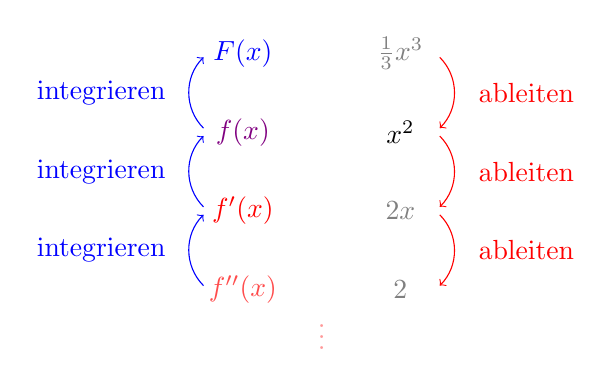
\begin{tikzpicture}
        \node[blue] at (0,1) {$F(x)$};
        \node[black!50!white] at (2,1) {$\frac{1}{3}x^3$};
        \node[violet] at (0,0) {$f(x)$};
        \node[black] at (2,0) {$x^2$};
        \node[red] at (0,-1) {$f'(x)$};
        \node[black!50!white] at (2,-1) {$2x$};
        \node[white!30!red] at (0,-2) {$f''(x)$};
        \node[black!50!white] at (2,-2) {$2$};
        \node[white!60!red] at (1,-2.5) {$\vdots$};
        \draw[blue,->] (-0.5,0.05) to[out=135, in=225] (-0.5,0.95);
        \draw[blue,->] (-0.5,-0.95) to[out=135, in=225] (-0.5,-0.05);
        \draw[blue,->] (-0.5,-1.95) to[out=135, in=225] (-0.5,-1.05);
        \draw[red,->] (2.5,-0.05) to[out=315, in=45] (2.5,-0.95);
        \draw[red,->] (2.5,-1.05) to[out=315, in=45] (2.5,-1.95);
        \draw[red,->] (2.5,0.95) to[out=315, in=45] (2.5,0.05);
        \node[blue] at (-1.8,0.5) {integrieren};
        \node[blue] at (-1.8,-0.5) {integrieren};
        \node[blue] at (-1.8,-1.5) {integrieren};
        \node[red] at (3.6,0.5) {ableiten};
        \node[red] at (3.6,-0.5) {ableiten};
        \node[red] at (3.6,-1.5) {ableiten};
    \end{tikzpicture}
\end{center}
Wenn wir die Stammfunktion einer Funktion in einer Formel aufschreiben möchten, dann können wir ein Integralzeichen ohne
festgelegte Grenzen verwenden:
\[F(x)=\frac{1}{3}x^3=\int x^2\diff x.\]
Das Integralzeichen beschreibt hier also keine Fläche (weil die Grenzen fehlen), sondern eine Stammfunktion.
\begin{example}{}
    Wir haben die Funktion $f(x)=2x$ und möchten diese \emph{integrieren}. Weiter oben siehst du, dass du $x^2$ ableiten
    kannst, um $2x$ zu erhalten. $F(x)=x^2$ ist somit eine Stammfunktion von $f(x)=2x$ und es gilt
    \[\int 2x\diff x=x^2.\]
\end{example}
Um beim Integrieren nicht immer raten zu müssen, überlegen wir uns nun ein paar Integrationsregeln, indem wir einige
bekannte Ableitungsregeln rückwärts anwenden. Wir fangen mit der Potenzregel an und können die folgende Regel beweisen.
\begin{theorem}{Potenzregel der Integration}
    Es sei $f(x)=x^n$ für ein $n\in\N$. Dann ist $F(x)=\frac{1}{n+1}x^{n+1}$ eine Stammfunktion von $f$.
\end{theorem}
\begin{proof}
    Wir leiten die Funktion $F(x)=\frac{1}{n+1}x^{n+1}$ ab, um zu überprüfen, dass die Regel gilt.
    \[\Bigl(\frac{1}{n+1}x^{n+1}\Bigr)'=\frac{1}{n+1}\cdot (n+1)x^n=x^n\]
    Hier haben wir erst die Potenzregel angewandt und anschließend $n+1$ gekürzt. $\frac{1}{n+1}x^{n+1}$ ist 
    also eine Stammfunktion von $x^n$.
\end{proof}
\begin{example}[ex:potenzintegration]{}
    Wir können mit der Potenzregel die folgenden Stammfunktionen bestimmen:
    \begin{itemize}
        \item $f(x)=x^4$ hat die Stammfunktion $\frac{1}{5}x^5$ (hier haben wir die Regel mit $n=4$ und $n+1=5$ verwendet).
        \item $f(x)=28x^6$ hat die Stammfunktion $28\cdot\frac{1}{7}x^7=4x^7$ (hier ist $n=6,n+1=7$).
    \end{itemize}
\end{example}
Wir wissen vom Ableiten außerdem, dass Konstanten immer verschwinden, d.h. die Ableitung einer konstanten Funktion wie
$f(x)=4$, $f(x)=13$ oder $f(x)=\pi$ ist stets $0$. Wenn wir eine Stammfunktion $F(x)$ gefunden haben und zu dieser Stammfunktion
einen konstanten Wert $c\in\R$ addieren, verschwindet dieser also beim Ableiten und unsere Funktion $F(x)+c$ bleibt eine
Stammfunktion.
\begin{example}{}
    Die Funktion $F(x)=x^2$ ist eine Stammfunktion von $f(x)=2x$. Wenn wir zu $F(x)$ nun einen konstanten Wert addieren --
    zum Beispiel 4 -- dann erhalten wir $F(x)+4=x^2+4$. Leiten wir diese neue Funktion ab, so erhalten wir mit der
    Summenregel die Ableitung
    \[(x^2+4)'=2x+0=2x.\]
    Die Funktion $F(x)+4=x^2+4$ ist also ebenfalls eine Stammfunktion von $f$.
\end{example}
Jede Funktion hat also unendlich viele Stammfunktionen. Haben wir nämlich eine Stammfunktion gefunden, so können wir
eine beliebige Zahl dazu addieren, um eine neue Stammfunktion zu bekommen.

Mit der Potenzregel der Integration und ein bisschen Wissen über Ableitungen kannst du bereits viele Stammfunktionen
ausrechnen. Hilfreich ist es oft, die Potenzregel der Integration in Kombination mit der Summen- und der Faktorregel
anzuwenden, also Summen einzeln zu integrieren und Vorfaktoren einfach in die Stammfunktion zu übernehmen. Zum Beispiel haben wir 
in Beispiel \ref{ex:potenzintegration} den Vorfaktor $28$ einfach in die Stammfunktion mitgenommen.
\begin{example}{}
    Es sei $f(x)=2x^3+\cos x+e^x$. Hier können wir die Summenregel ($*$) verwenden und, statt die gesamte Funktion auf einmal
    zu integrieren, die Funktionen $2x^3$, $\cos x$ und $e^x$ einzeln integrieren:
    \[F(x)=\int2x^3+\cos x+e^x\diff x\stackrel{(*)}{=}\int 2x^3\diff x+\int\cos x\diff x+\int e^x\diff x\]
    Mit der Potenzregel erhalten wir für die erste Funktion die Stammfunktion $\frac{1}{2}x^4$. Vielleicht erinnerst du 
    dich noch daran, dass die Ableitung von $\sin x$ die Funktion $\cos x$ ist (siehe Seite \pageref{ableitung-trigonometrie}).
    Eine Stammfunktion von $\cos x$ ist also $\sin x$.

    Schließlich ist die Ableitung von $e^x$ wieder $e^x$ (siehe Seite \pageref{ableitung-exponentialfunktion}). Eine
    Stammfunktion von $e^x$ ist also wieder $e^x$. Insgesamt bringt uns das die Stammfunktion
    \[F(x)=\int 2x^3\diff x+\int\cos x\diff x+\int e^x\diff x=\frac{1}{2}x^4+\sin x+e^x.\]
\end{example}

\begin{advanced}{Partielle Integration und Integration durch Substitution}
    Ebenso wie die Potenzregel lässt sich auch die Produkt- und die Kettenregel rückwärts anwenden, um weitere Regeln für das Integrieren
    von Funktionen zu erhalten. Wie genau das geht und wie du diese Regeln anwenden kannst, um kompliziertere Funktionen 
    integrieren zu können (die du sonst nur durch Raten integrieren kannst), erfährst du auf Seite 
    \pageref{partielle-integration} (für partielle Integration) bzw. 
    \pageref{substitution} (für Integration durch Substitution).
\end{advanced}
Was haben Stammfunktionen nun aber mit Integralen zu tun und wie können sie uns helfen, Integrale \emph{ohne}
die Verwendung von Rechtecken auszurechnen? Eine Antwort darauf liefert der Hauptsatz der Differential- und 
Integralrechnung. 
\begin{theorem}{Hauptsatz der Differential- und Integralrechnung}
    Sei $f:[a,b]\rightarrow\mathbb{R}$ stetig und $F$ eine Stammfunktion von $f$. Dann gilt
    \[\int_a^b f(x)~dx=F(b)-F(a)=:\Bigl[F(x)\Bigr]_a^b\]
\end{theorem}
\begin{example}{}
    Der Hauptsatz der Differential- und Integralrechnung gibt uns die Möglichkeit, die aufwendige Berechnung eines
    Flächeninhalts zu umgehen, indem wir einfach eine Stammfunktion bestimmen. Wenn wir das Integral
    \[\int_2^52x\diff x\]
    ausrechnen möchten, dann müssen wir zunächst die Stammfunktion von $f(x)=2x$ bestimmen. Wir erhalten das Ergebnis
    $F(x)=x^2$. Nun müssen wir die Integralgrenzen $a=2$ und $b=5$ noch in die Stammfunktion einsetzen und es gilt
    \[\int_2^52x\diff x=F(b)-F(a)=5^2-2^2=25-4=21.\]
\end{example}
Wenn wir ein Integral
\[\int_a^bf(x)\diff x\]
berechnen möchten, müssen wir zunächst eine Stammfunktion $F(x)$ von $f(x)$ berechnen. Anschließend liefert uns der Satz, dass
wir nur noch
\[F(b)-F(a)\]
ausrechnen müssen. Wichtig ist, dass $b$ hier die obere (also rechte) Integralgrenze und $a$ die untere (also linke) 
Grenze ist. Wir dürfen diese Grenzen nicht vertauschen, weil das Ergebnis sonst das falsche Vorzeichen hat.
Die Schreibweise
\[\Bigl[F(x)\Bigr]_a^b\]
ist eine Abkürzung für die Differenz $F(b)-F(a)$, die wir immer ausrechnen müssen, wenn wir ein Integral bestimmen wollen.
\begin{advanced}{Beweis zum Hauptsatz der Differential- und Integralrechnung}
    Eine vollständige Herleitung des obigen Satzes würde den Rahmen dieses Abschnitts sprengen. Du kannst die
    gesamte Herleitung aber auf Seite \pageref{hdi-beweis} finden.
\end{advanced}
Dies ist ein wirklich mächtiges Werkzeug, denn es reduziert die Aufgabe, Flächen zu berechnen, darauf, eine Stammfunktion
zu bestimmen. Wenn wir ein Integral ausrechnen wollen, besteht die eigentliche Aufgabe also darin, Stammfunktionen zu
bestimmen.
\begin{example}{}
    \parpic[r]{
    \begin{tikzpicture}
        \begin{axis}[
            defgrid, y=1cm, x=1cm, ymin=0, ymax=4, xmin=0, xmax=4, xtick={1,...,4}, ytick={1,...,4}
            ]
            \addplot[name path=poly, domain=1:4, violet] {0.33333*(x-1)*(x-4)*(x-6)};
            \addplot[name path=line, domain=1:4, violet] {0};
            \addplot[fill opacity=0.5, fill=violet!20] fill between[ 
            of = poly and line,
            soft clip={domain=1:4},
            ];
        \end{axis}
    \end{tikzpicture}
    }
    Wir können jetzt den Flächeninhalt der Fläche aus der Einführung berechnen, die du rechts noch einmal siehst. Die
    Fläche ist nach oben durch die Funktion
    \[f(x)=\frac{(x-1)(x-4)(x-6)}{3}\]
    beschränkt. Wir müssen also
    \[\int_1^4\frac{(x-1)(x-4)(x-6)}{3}\diff x\]
    bestimmen. Dazu benötigen wir zunächst die Stammfunktion von $f$. Wir können den Term im Zähler Ausmultiplizieren:
    \[(x-1)(x-4)(x-6)=(x^2-5x+4)(x-6)=x^3-11x^2+34x-24\]
    Mit der Potenzregel der Integration erhalten wir die Stammfunktion
    \[F(x)=\frac{\frac{1}{4}x^4-\frac{11}{3}x^3+17x^2-24x}{3}=\frac{1}{12}x^4-\frac{11}{9}x^3+\frac{17}{3}x^2-8x.\]
    Jetzt können wir den Hauptsatz der Differential- und Integralrechnung verwenden und das Integral ausrechnen:
    \begin{align*}
        &\int_1^4\frac{(x-1)(x-4)(x-6)}{3}\diff x=\Biggl[\frac{1}{12}x^4-\frac{11}{9}x^3+\frac{17}{3}x^2-8x\Biggr]_1^4\\
        =&\frac{1}{12}\cdot 4^4-\frac{11}{9}\cdot 4^3+\frac{17}{3}\cdot 4^2-8\cdot 4-\Biggl(\frac{1}{12}\cdot 1^4-\frac{11}{9}\cdot 1^3+\frac{17}{3}\cdot 1^2-8\cdot 1\Biggr)\\
        =&\frac{64}{3}-\frac{704}{9}+\frac{272}{3}-32-\frac{1}{12}+\frac{11}{9}-\frac{17}{3}+8\\
        =&\frac{192}{9}-\frac{704}{9}+\frac{816}{9}+\frac{11}{9}-\frac{51}{9}-32+8-\frac{1}{12}\\
        =&\frac{264}{9}-24-\frac{1}{12}
        =\frac{264}{9}-\frac{216}{9}-\frac{1}{12}
        =\frac{48}{9}-\frac{1}{12}\\
        =&\frac{16}{3}-\frac{1}{12}
        =\frac{64}{12}-\frac{1}{12}
        =\frac{63}{12}=5.25\\
    \end{align*}
    Die eingezeichnete Fläche hat also einen Flächeninhalt von $5.25$. Das konnten wir trotz der Krümmung berechnen.
\end{example}
\begin{nutshell}{Der Hauptsatz der Differential- und Integralrechnung}
    Eine differenzierbare Funktion $F(x)$ wird als \textbf{Stammfunktion} einer Funktion $f(x)$ bezeichnet, 
    wenn $f(x)$ die Ableitung von $F(x)$ ist. Die Stammfunktion einer Funktion $f(x)$ schreiben wir auch als
    \[F(x)=\int f(x)\diff x.\]
    Wir lassen die Grenzen des Integrals weg, um zu symbolisieren, dass wir keine Fläche, sondern die Stammfunktion
    meinen. Wenn wir zu einer Funktion die Stammfunktion berechnen, sagen wir auch, dass wir die Funktion
    \textbf{integrieren}. Mithilfe der Stammfunktion lassen sich Integrale ohne Rechtecksummen berechnen. Ist nämlich $F(x)$
    eine Stammfunktion von $f(x)$, so ist
    \[\int_a^b f(x)~dx=F(b)-F(a)=:\Bigl[F(x)\Bigr]_a^b.\]
\end{nutshell}
\end{document}